\section{Les médias}
\subsection{Format des images}
\begin{frame}{Les images matricielles (bitmap)}
  \begin{itemize}
  \item[\dialoginformation] Les images issues du processus de discrétisation
    sont décomposés en \emph{pixels} (souvent rectangulaires).
  \item[\ddialogwarning] les formats RAW (qui contiennent les données brutes
    issues des capteurs d'appareils photo) ont des grilles qui sont plutôt des
    pavages par des triangles ou des hexagones.
  \end{itemize}
  Une image est un format \emph{composite}. Il contient entre autres:
  \begin{itemize}
  \item La largeur et la hauteur en pixels (obligatoire)
  \item Les données d'intensité de chaque pixel (obligatoire)
  \item Des informations sur le rendu des couleurs (voir plus loin, le gamma
    et le gamut)
  \item Des informations sur le rendu physique (par exemple, tailles en cm)
  \item Des méta-données (sujet, auteur, lieu de prise)
  \end{itemize}
\end{frame}
\begin{frame}[fragile]{Le format PBM}
  \begin{columns}
    \begin{column}{0.7\linewidth}
      Le format PBM est un format matriciel qui est composé des éléments
      suivants:
      \begin{itemize}
      \item une entête en mode texte qui commence par P4 en ASCII, du blanc
      \item la largeur écrite en ASCII, du blanc
      \item la hauteur écrite en ASCII, \textbf{un} blanc
      \item Les données binaires ligne par ligne de haut en bas.
      \item Chaque ligne est découpée en paquet de 8 pixels noirs ou blancs
        consécutifs, codés en binaire (1=noir). Si la largeur n'est pas un
        multiple de 8, on complète par des 0 à droite.
      \end{itemize}
    \end{column}%
    \begin{column}{0.3\linewidth}
      \begin{center}
        \begin{tikzpicture}[baseline={([yshift={-\ht\strutbox}]current
            bounding box.north)},scale=.15]
          \draw[solarizedRebase03,thick] (0,0) rectangle (16,16);
          \draw[solarizedRebase0,very thin] (0,0) grid (16,16); \foreach \i in
          {(5,0),(6,0),(7,0),(8,0),(9,0),(10,0),(12,0),(13,0),(14,0),(2,1),%
            (3,1),(4,1),(5,1),(6,1),(7,1),(8,1),(9,1),(10,1),(11,1),(12,1),(13,1),%
            (2,2),(3,2),(5,2),(8,2),(9,2),(10,2),%
            (2,3),(3,3),(4,3),(8,3),(9,3),(10,3),%
            (1,4),(2,4),(4,4),(8,4),(10,4),%
            (2,5),(4,5),(8,5),(10,5),(1,6),(4,6),(7,6),(10,6),(11,6),%
            (1,7),(5,7),(6,7),(12,7),(1,8),(13,8),(1,9),(13,9),(2,10),(13,10),%
            (3,11),(13,11),(3,12),(7,12),(10,12),(14,12),(15,12),%
            (4,13),(7,13),(9,13),(11,13),(13,13),(15,13),%
            (5,14),(6,14),(8,14),(9,14),(12,14),(14,14),(13,15)} {%
            \fill[fill=solarizedRebase1] \i rectangle ++(1,1); }%
          \only<3|handout:0>{%
            \draw[solarizedRebase3,thick] (0,15) rectangle (8,16); }%
          \only<4|handout:0>{%
            \draw[solarizedRebase3,thick] (8,15) rectangle (16,16); }%
          \only<5|handout:0>{%
            \draw[solarizedRebase3,thick] (0,14) rectangle (8,15); }%
        \end{tikzpicture}
      \end{center}
      L'entête en ASCII:
      \begin{center}
        \framebox{\begin{minipage}{.8\linewidth}\ttfamily%
            \textcolor<2>{solarizedRebase3}{P4\textbackslash n\\
              16 16\textbackslash n}
          \end{minipage}}
      \end{center}
    \end{column}
  \end{columns}
  \begin{center}
    \framebox{\begin{minipage}{.9\linewidth}\ttfamily%
        ADRESSE~~~OCTETS EN HEXADECIMAL\\
        00000000~~\textcolor<2>{solarizedRebase3}{50 34 0a 31 36 20 31 36 0a} \textcolor<3>{solarizedRebase3}{00} \textcolor<4>{solarizedRebase3}{04} \textcolor<5>{solarizedRebase3}{06} ca 09 55 11\\
        00000010~~23 10 04 20 04 40 04 40 04 46 08 49 30 28 a0 68\\
        00000020~~a0 38 e0 34 e0 3f fc 07 ee
      \end{minipage}}
  \end{center}
\end{frame}
\begin{exercice}
  \begin{exercicelet}{Décodage d'un fichier PBM}
    Voici la séquence d'octets qui compose un fichier PBM:\\
    \texttt{50 34 0a 38 20 31 30 0a 41 41 3e 55 41 49 bf 12 24 22}
    \begin{questions}
    \item Repérez l'entête du fichier, et traduisez-là en ASCII.
      \begin{correction}
        \texttt{P4(retour chariot)8(espace)10(retour chariot)}
      \end{correction}
    \item Quelle est la taille de cette image (en pixels) ?
      \begin{correction}
        8 par 10
      \end{correction}
    \item Dessinez le fichier résultant.
      \begin{correction}
        
\includegraphics[width=3cm]{img/06/alien.png}
      \end{correction}
    \item Quelle est la taille (minimale) de l'entête et la taille des données
      ?
      \begin{correction}
        $5+2\times 1=7$ pour l'entête et $10$ octets pour les données
      \end{correction}
    \item Même question pour une image 8000 par 8000.
      \begin{correction}
        $5+2\times 4=13$ pour l'entête et $8000000$ octets pour les
        données. L'entête est donc négligeable.
      \end{correction}
    \end{questions}
  \end{exercicelet}
\end{exercice}
\begin{frame}{Le format JPG}
  \begin{itemize}
  \item Format développé par comité \emph{(Joint Picture Expert Group)}
  \item Adapté au stockage de photographies
  \item Méta-données riches (EXIF, XMP, ITPC)
  \item Filtrage perceptuel numérique: on enlève des couleurs (filtrage
    haute-fréquences)
  \item Compression sur un filtrage plus ou moins intense
  \item Stockage avec perte de qualité
  \end{itemize}
  \begin{columns}
    \begin{column}{.33\linewidth}\centering
      \includegraphics<1|handout:1>[width=\linewidth]{img/06/lena90}
      \includegraphics<2|handout:2>[width=\linewidth]{img/06/zoom90} \\Lena,
      90\%, 90 ko
    \end{column}%
    \begin{column}{.33\linewidth}\centering
      \includegraphics<1|handout:1>[width=\linewidth]{img/06/lena50}
      \includegraphics<2|handout:2>[width=\linewidth]{img/06/zoom50} \\Lena,
      50\%, 30 ko
    \end{column}%
    \begin{column}{.33\linewidth}\centering
      \includegraphics<1|handout:1>[width=\linewidth]{img/06/lena10}
      \includegraphics<2|handout:2>[width=\linewidth]{img/06/zoom10} \\Lena,
      10\%, 10 ko
    \end{column}%
  \end{columns}
  \vfill
\end{frame}
\begin{frame}{Le format PNG}
  \begin{itemize}
  \item Format \emph{Portable Network Graphics}
  \item Méta-données liées aux couleurs
  \item Pas de filtrage perceptuel numérique
  \item Compression tenant compte de l'aspect 2D
  \item Support de la transparence et de la translucidité (transparence
    partielle)
  \item Support d'une palette de couleurs: les données colorimétriques de
    chaque point sont regroupées dans une palette unique, et on ne note que le
    numéro de couleur dans la palette pour chaque point.
  \end{itemize}
  \begin{columns}
    \begin{column}{.33\linewidth}\centering
      \includegraphics<1|handout:1>[width=\linewidth]{img/01/lena.png}
      \includegraphics<2|handout:2>[width=\linewidth]{img/06/zoom} \\Lena, 475
      ko
    \end{column}%
    \begin{column}{.33\linewidth}\centering
      \includegraphics<1|handout:1>[width=\linewidth]{img/06/lena256}
      \includegraphics<2|handout:2>[width=\linewidth]{img/06/zoom256} \\Lena,
      palette 256c, 189 ko
    \end{column}%
    \begin{column}{.33\linewidth}\centering
      \includegraphics<1|handout:1>[width=\linewidth]{img/06/lena4}
      \includegraphics<2|handout:2>[width=\linewidth]{img/06/zoom4} \\Lena,
      palette 4c, 50 ko
    \end{column}%
  \end{columns}
  \vfill
\end{frame}
\begin{frame}[fragile]{Les images vectorielles}
  \begin{itemize}
  \item Les images vectorielles sont stockées sous forme de courbes
    mathématiques: points, traits, courbes.
  \item Courbes de Bézier: équations polynomiales de degré 2 ou 3, déterminées
    par des points d'ancrage (1+degré) qui «~passe entre les points~»
    \url{http://en.wikipedia.org/wiki/Bezier_curve}
  \item Précision arbitraire
  \item Gestion du texte
  \item Adapté aux images synthétiques (dessins avec aplats)
  \end{itemize}
  \begin{columns}
    \begin{column}{.33\linewidth}\centering
      
\includegraphics[width=\linewidth]{img/06/tiger512}\\Tigre, zoom ×1
    \end{column}%
    \begin{column}{.33\linewidth}\centering
      
\includegraphics[width=\linewidth]{img/06/tiger4096}\\Tigre, zoom ×64
    \end{column}%
    \begin{column}{.33\linewidth}\centering
      
\includegraphics[width=\linewidth]{img/06/tiger32768}\\Tigre, zoom ×4096
    \end{column}%
  \end{columns}
\end{frame}
\begin{frame}{Le format SVG}
  \begin{columns}
    \begin{column}{.5\linewidth}
      \begin{itemize}
      \item Le format SVG est un format en mode texte qui décrit des images
        vectorielles.
      \item Des balises faites avec < et > délimitent les éléments
      \item On décrit les courbes par leurs coordonnées
      \item Métadonnées en XML possibles
      \item Visualisables directement dans les navigateurs
      \end{itemize}
    \end{column}
    \begin{column}{.5\linewidth}
      \begin{tikzpicture}[scale=.02]
\draw[thin] (0,0) rectangle (300,200);
\fill[green] (0,70) rectangle ++(100,80);
\draw[red,thick] (5,5)--(250,95);
\fill[blue] (90,80) circle (50);
\node [inner sep=0pt,outer sep=0pt,anchor=south west] at (180,60) {Un texte};
\end{tikzpicture}
    \end{column}
  \end{columns}
  \lstinputlisting[language=XML]{img/06/test.svg}
\end{frame}
\begin{exercice}
  \begin{exercicelet}{Choix de format d'image}
    \begin{questions}
    \item Voici quatre images. Imaginez le format le plus adapté à chacune
      d'entre elles. Expliquez votre choix.\\
      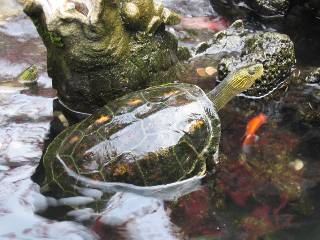
\includegraphics[width=.2\linewidth]{img/06/tortue.jpg} \hfill
      
\includegraphics[width=.2\linewidth]{img/common/dialog-system.png}
      \hfill
      \begin{tikzpicture}[scale=.2,outer sep=0pt, edges/.style={very thin},%
        ]
        \def\vertex#1#2#3{\coordinate #2 at #3;\fill #2 circle (5pt)}%
        \vertex{125}{(noeud1100100)}{(25.63377pt,12.3443pt)};
        \vertex{145}{(noeud1001100)}{(6.33083pt,27.73811pt)};
        \vertex{147}{(noeud1001001)}{(-17.7391pt,22.2439pt)};
        \vertex{347}{(noeud0011001)}{(-28.4523pt,0.0pt)};
        \vertex{367}{(noeud0010011)}{(-17.73868pt,-22.2439pt)};
        \vertex{236}{(noeud0110010)}{(6.3304pt,-27.73856pt)};
        \vertex{256}{(noeud0100110)}{(25.63377pt,-12.34474pt)};
        \vertex{267}{(noeud0100011)}{(61.7215pt,128.16666pt)};
        \vertex{235}{(noeud0110100)}{(-61.7215pt,128.16887pt)};
        \vertex{156}{(noeud1000110)}{(-138.69057pt,31.652pt)};
        \vertex{124}{(noeud1101000)}{(-111.21948pt,-88.69339pt)};
        \vertex{457}{(noeud0001101)}{(0.0pt,-142.2615pt)};
        \vertex{137}{(noeud1010001)}{(111.21948pt,-88.69553pt)};
        \vertex{346}{(noeud0011010)}{(138.69278pt,31.652pt)};
        \vertex{127}{(noeud1100001)}{(15.82706pt,69.34528pt)};
        \vertex{345}{(noeud0011100)}{(-44.34776pt,55.60974pt)};
        \vertex{167}{(noeud1000011)}{(-71.13075pt,0.0pt)};
        \vertex{234}{(noeud0111000)}{(-44.3467pt,-55.60974pt)};
        \vertex{567}{(noeud0000111)}{(15.82599pt,-69.34639pt)};
        \vertex{123}{(noeud1110000)}{(64.08443pt,-30.86185pt)};
        \vertex{456}{(noeud0001110)}{(64.08443pt,30.86075pt)};
        \vertex{467}{(noeud0001011)}{(111.21948pt,88.69339pt)};
        \vertex{237}{(noeud0110001)}{(0.0pt,142.2615pt)};
        \vertex{356}{(noeud0010110)}{(-111.21948pt,88.69553pt)};
        \vertex{126}{(noeud1100010)}{(-138.69278pt,-31.65413pt)};
        \vertex{245}{(noeud0101100)}{(-61.7215pt,-128.16887pt)};
        \vertex{157}{(noeud1000101)}{(61.7215pt,-128.16887pt)};
        \vertex{134}{(noeud1011000)}{(138.69057pt,-31.65413pt)};
        \vertex{135}{(noeud1010100)}{(97.56273pt,122.34378pt)};
        \vertex{146}{(noeud1001010)}{(-34.81718pt,152.56206pt)};
        \vertex{247}{(noeud0101001)}{(-140.98332pt,67.89365pt)};
        \vertex{357}{(noeud0010101)}{(-140.98575pt,-67.89365pt)};
        \vertex{136}{(noeud1010010)}{(-34.81718pt,-152.55962pt)};
        \vertex{246}{(noeud0101010)}{(97.56508pt,-122.34143pt)};
        \vertex{257}{(noeud0100101)}{(156.48766pt,0.0pt)};
        \draw[edges](noeud1100100)--(noeud0011001);
        \draw[edges](noeud1100100)--(noeud0010011); \draw[edges]
        (noeud1100100)..controls (82.98134pt,12.0355pt)..(noeud0011010);
        \draw[edges] (noeud1100100)..controls
        (61.1481pt,57.37003pt)..(noeud0001011);
        \draw[edges](noeud1001100)--(noeud0010011);
        \draw[edges](noeud1001100)--(noeud0110010); \draw[edges]
        (noeud1001100)..controls (42.32513pt,72.38084pt)..(noeud0100011);
        \draw[edges] (noeud1001100)..controls
        (-6.72974pt,83.58076pt)..(noeud0110001);
        \draw[edges](noeud1001001)--(noeud0110010);
        \draw[edges](noeud1001001)--(noeud0100110); \draw[edges]
        (noeud1001001)..controls (-30.19975pt,78.22093pt)..(noeud0110100);
        \draw[edges] (noeud1001001)..controls
        (-69.53915pt,46.84906pt)..(noeud0010110);
        \draw[edges](noeud0011001)--(noeud0100110); \draw[edges]
        (noeud0011001)..controls (-79.98648pt,25.15688pt)..(noeud1000110);
        \draw[edges] (noeud0011001)..controls
        (-79.9874pt,-25.15811pt)..(noeud1100010); \draw[edges]
        (noeud0010011)..controls (-69.53874pt,-46.84798pt)..(noeud1101000);
        \draw[edges] (noeud0010011)..controls
        (-30.19952pt,-78.22096pt)..(noeud0101100); \draw[edges]
        (noeud0110010)..controls (-6.72992pt,-83.58104pt)..(noeud0001101);
        \draw[edges] (noeud0110010)..controls
        (42.32506pt,-72.38211pt)..(noeud1000101); \draw[edges]
        (noeud0100110)..controls (61.14795pt,-57.37129pt)..(noeud1010001);
        \draw[edges] (noeud0100110)..controls
        (82.9804pt,-12.03697pt)..(noeud1011000);
        \draw[edges](noeud0100011)--(noeud0011100);
        \draw[edges](noeud0100011)--(noeud1011000);
        \draw[edges](noeud0100011)--(noeud1010100);
        \draw[edges](noeud0110100)--(noeud1000011);
        \draw[edges](noeud0110100)--(noeud0001011);
        \draw[edges](noeud0110100)--(noeud1001010);
        \draw[edges](noeud1000110)--(noeud0111000);
        \draw[edges](noeud1000110)--(noeud0110001);
        \draw[edges](noeud1000110)--(noeud0101001);
        \draw[edges](noeud1101000)--(noeud0000111);
        \draw[edges](noeud1101000)--(noeud0010110);
        \draw[edges](noeud1101000)--(noeud0010101);
        \draw[edges](noeud0001101)--(noeud1110000);
        \draw[edges](noeud0001101)--(noeud1100010);
        \draw[edges](noeud0001101)--(noeud1010010);
        \draw[edges](noeud1010001)--(noeud0001110);
        \draw[edges](noeud1010001)--(noeud0101100);
        \draw[edges](noeud1010001)--(noeud0101010);
        \draw[edges](noeud0011010)--(noeud1100001);
        \draw[edges](noeud0011010)--(noeud1000101);
        \draw[edges](noeud0011010)--(noeud0100101);
        \draw[edges](noeud1100001)--(noeud0011100);
        \draw[edges](noeud1100001)--(noeud0001110);
        \draw[edges](noeud1100001)--(noeud0010110);
        \draw[edges](noeud0011100)--(noeud1000011);
        \draw[edges](noeud0011100)--(noeud1100010);
        \draw[edges](noeud1000011)--(noeud0111000);
        \draw[edges](noeud1000011)--(noeud0101100);
        \draw[edges](noeud0111000)--(noeud0000111);
        \draw[edges](noeud0111000)--(noeud1000101);
        \draw[edges](noeud0000111)--(noeud1110000);
        \draw[edges](noeud0000111)--(noeud1011000);
        \draw[edges](noeud1110000)--(noeud0001110);
        \draw[edges](noeud1110000)--(noeud0001011);
        \draw[edges](noeud0001110)--(noeud0110001);
        \draw[edges](noeud0001011)--(noeud1010100);
        \draw[edges](noeud0110001)--(noeud1001010);
        \draw[edges](noeud0010110)--(noeud0101001);
        \draw[edges](noeud1100010)--(noeud0010101);
        \draw[edges](noeud0101100)--(noeud1010010);
        \draw[edges](noeud1000101)--(noeud0101010);
        \draw[edges](noeud1011000)--(noeud0100101); \draw[edges]
        (noeud1010100)..controls (-47.76291pt,209.26231pt)..(noeud0101001);
        \draw[edges] (noeud1010100)..controls
        (214.64177pt,0.0026pt)..(noeud0101010); \draw[edges]
        (noeud1001010)..controls (-193.38428pt,93.13577pt)..(noeud0010101);
        \draw[edges] (noeud1001010)..controls
        (133.83827pt,167.81918pt)..(noeud0100101); \draw[edges]
        (noeud0101001)..controls (-193.3816pt,-93.13309pt)..(noeud1010010);
        \draw[edges] (noeud0010101)..controls
        (-47.763pt,-209.25972pt)..(noeud0101010); \draw[edges]
        (noeud1010010)..controls (133.83827pt,-167.8165pt)..(noeud0100101);
      \end{tikzpicture}\hfill
      
\includegraphics[width=.2\linewidth]{img/06/home_organization}

      \begin{xcorrection}
        JPEG (photo), PNG (mais pixelisé) ou vectoriel pour un icone,
        Vectoriel, PNG (peu de couleurs: palette petite, compression idéale,
        dessin au trait pas idéal en JPG).
      \end{xcorrection}
    \end{questions}
  \end{exercicelet}
  \begin{exercicelet}{Palette}
    \begin{questions}
    \item Une image 1000×1000 utilise 3 octets pour décrire la couleur de
      chaque pixel. Calculez la taille occupée par les données de cette image
      en PNG.
      \begin{xcorrection}
        3 Mo
      \end{xcorrection}
    \item Cette image n'a que 256 couleurs au total. On peut utiliser une
      palette de couleurs. Calculez la taille de la palette et la taille des
      données de l'image utilisant la palette.
      \begin{xcorrection}
        1 Mo+768 o pour la palette
      \end{xcorrection}
    \end{questions}
  \end{exercicelet}
\end{exercice}
\subsection{Les couleurs}
\begin{frame}{Qu'est-ce qu'une couleur?}
  \begin{itemize}
  \item Réaction du cerveau à l'intensité des longueurs d'ondes de la lumière
  \item Certaines longueurs d'onde ne sont pas visibles
  \item Le mélange de longueurs d'onde est vu comme une autre couleur.
  \item Certaines couleurs ne sont obtensibles que par mélange (rose, marron)
  \item On distingue la couleur d'une source lumineuse, et la couleur d'un
    objet éclairé.
  \item[\ddialogwarning] Un objet absorbe une partie de la lumière et recrache
    le reste. Par exemple, la chlorophylle absorbe essentiellement tout sauf
    le vert.
  \item Les couleurs d'une source s'additionnent: synthèse additive
  \item Les couleurs de pigments se masquent mutuellement: synthèse
    soustractive
  \end{itemize}
  \begin{center}
    
\includegraphics[width=.8\linewidth]{img/06/Spectrum_roygbiv.jpg}
  \end{center}
\end{frame}
\begin{frame}{Le gamut: teinte et saturation}
  \begin{columns}
    \begin{column}{.5\linewidth}
      \begin{itemize}
      \item Une couleur peut être définie par sa teinte (ou ton), sa
        saturation (intensité de la teinte) et sa luminosité.
      \item Le gamut représente l'étendue des couleurs qui peuvent être
        reproduites par un moniteur ou une imprimante à luminosité fixée
      \item Le polygone représente les couleurs que l'on peut reproduire ; les
        extrémités sont les tons des couleurs de base que l'on mélange.
      \item[\ddialogerror] Certaines couleurs ne peuvent pas être obtenues. On
        perd de l'information lorsqu'on passe d'un système à un autre.
      \item[\ddialoginformation] On utilise des profils couleurs ICC pour
        représenter le gamut et assurer les meilleures conversions possibles.
      \end{itemize}
    \end{column}%
    \begin{column}{.5\linewidth}
      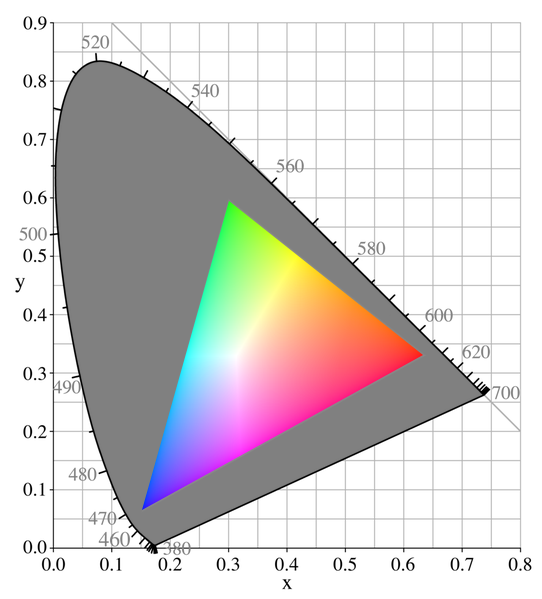
\includegraphics[width=\linewidth]{img/06/CIExy1931_srgb_gamut}
    \end{column}
  \end{columns}
\end{frame}
\begin{frame}{Le gamma: luminance}
  \begin{itemize}
  \item La luminance est l'intensité de la couleur produite
  \item Le facteur $\gamma$ caractérise la réponse lumineuse au stimulus
    électrique: $I=kV^\gamma$.
  \item[\dialogwarning] C'est donc un coefficient d'une réponse exponentielle.
  \end{itemize}
  \begin{center}\renewcommand{\tabcolsep}{1mm}\color{red}
    \begin{tabular}{cccccccccccc}
      Intensité &
      \cellcolor[gray]{.0} 0\%&
      \cellcolor[gray]{.39} 39\%&
      \cellcolor[gray]{.52} 52\%&
      \cellcolor[gray]{.61} 61\%&
      \cellcolor[gray]{.69} 69\%&
      \cellcolor[gray]{.75} 75\%&
      \cellcolor[gray]{.81} 81\%&
      \cellcolor[gray]{.86} 86\%&
      \cellcolor[gray]{.91} 91\%&
      \cellcolor[gray]{.95} 95\%&
      \cellcolor[gray]{1} 100\%\\
      Codage &
      \cellcolor[gray]{.0} 0\% &
      \cellcolor[gray]{.1} 10\% &
      \cellcolor[gray]{.2} 20\% &
      \cellcolor[gray]{.3} 30\% &
      \cellcolor[gray]{.4} 40\% &
      \cellcolor[gray]{.5} 50\% &
      \cellcolor[gray]{.6} 60\% &
      \cellcolor[gray]{.7} 70\% &
      \cellcolor[gray]{.8} 80\% &
      \cellcolor[gray]{.9} 90\% &
      \cellcolor[gray]{1} 100\%\\
    \end{tabular}\\
    \color{solarizedRebase3}\small\itshape
    Signification: lorsque le signal d'entrée est de 10\% de la puissance
    maximale, la perception du gris est de 39\% environ. On compense donc le
    signal entré par le $\gamma$ inverse pour donner l'impression d'une
    progression linéaire.
  \end{center}
  \begin{itemize}
  \item Gamma normalisé des moniteurs: 2,5
  \item[\dialogerror] Mais... tous les moniteurs n'ont pas le même $\gamma$.
  \item Nécessité de corriger la correction (on fait le produit des $\gamma$).
  \end{itemize}
\end{frame}
\begin{frame}[fragile]{Images RVB (RGB en anglais)}
  \begin{columns}
    \begin{column}{.6\linewidth}
      \begin{itemize}
      \item Depuis le début de la conception des moniteurs, le standard est de
        recomposer la couleur par synthèse additive de 3 couleurs.
      \item On mesure les couleurs par l'intensité de chacune des couleurs
        primaires: rouge, vert et bleu
      \item On obtient des couleurs par mélange de différentes intensités
      \item Un système équivalent permet de désigner les couleurs par teinte,
        saturation et luminance relative (valeur): TSV (en anglais HSB,
        Hue/Saturation/Brightness).
      \item On utilise très souvent un octet d'information pour chaque
        composante.
      \item Notation usuelle: \#RRVVBB (avec chaque paire de lettre qui est un
        octet noté en hexadécimal).
      \end{itemize}
    \end{column}%
    \begin{column}{.4\linewidth}\centering
      \begin{tikzpicture}[scale=.5]
        \foreach \x in {0,0.0111,...,1} { \definecolor{currentcolor}{hsb}{\x,
            1, 1} \draw[draw=none, fill=currentcolor] (-360*\x+88:2) --
          (-360*\x+88:3.8) -- (-360*\x+92:3.8) -- (-360*\x+92:2) -- cycle; }
        \foreach \x/\y in
        {0/rouge,60/jaune,120/vert,180/cyan,240/bleu,300/magenta} { \draw
          [black] (90-\x:3.8)--(90-\x:5); \draw [decorate,decoration={text
            along path, text=\x{°}/\y}] (88-\x:4) arc (88-\x:28-\x:4); }
      \end{tikzpicture}
      \\
      La roue des couleurs permet d'identifier la teinte à saturation
      maximale.
    \end{column}
  \end{columns}
\end{frame}
\begin{exercice}
  \begin{exercicelet}{Décomposition de couleurs}
    Donnez des composantes couleur plausibles RGB des couleurs
    suivantes. Utilisez la notation HTML.
    \begin{itemize}
    \item Rouge, vert, bleu
    \item Cyan, magenta, jaune
    \item Blanc, noir
    \item Gris 50\%
    \item Marron foncé, rose pâle, orange vif
    \end{itemize}
    \begin{xcorrection}
      FF0000, 00FF00, 0000FF\\
      00FFFF, FF00FF, FFFF00\\
      FFFFFF, 000000\\
      808080\\
      200000 (ou autre faible quantité de rouge), FFE0E0 (rouge un peu plus
      que les autres, mais très blanc), FF7F00 (ou autre chose équivalente:
      mélange jaune+rouge)
    \end{xcorrection}
  \end{exercicelet}
  \begin{exercicelet}{Scanner}
    Un scanner scanne en RGB à une résolution de 1200 points par pouce (dans
    les deux directions). Pour simplifier, on considérera qu'il y a une
    surface de 10 pouces × 6 pouces scannable. Chaque couleur est scannée en
    12 bits. Quelle est la quantité d'information résultant de chaque scan ?
    \begin{xcorrection}
      1200×1200×60×12×3=3 110 400 000 soit environ 389 Mo.
    \end{xcorrection}
  \end{exercicelet}
\end{exercice}
\begin{frame}{Images CMJN et polychromes}
  \begin{columns}
    \begin{column}{.8\linewidth}
      \begin{itemize}
      \item L'impression utilise un standard de synthèse soustractive
      \item Deux pigments ensemble absorbent tous les deux la lumière et dans
        l'absolu le mélange complet fait du noir.
      \item[\dialogerror] Le noir par addition n'est pas assez noir, on
        utilise donc une encre noire pure.
      \item Utilisation des couleurs complémentaires cyan, magenta et jaune
      \item Standard de l'impression: la \emph{quadrichromie} CMJN (CMYK en
        anglais).
      \item[\dialogerror] Certaines teintes ne sont pas possibles: rose vif,
        oranges vifs.
      \item Possibilité d'impression pentachrome ou hexachrome
      \item[\ddialogwarning] possibilité de faire des couleurs garanties avec
        une encre par couleur sans mélanges: gamme Pantone® ou Focoltone®.
      \end{itemize}
    \end{column}%
    \begin{column}{.15\linewidth}\centering
      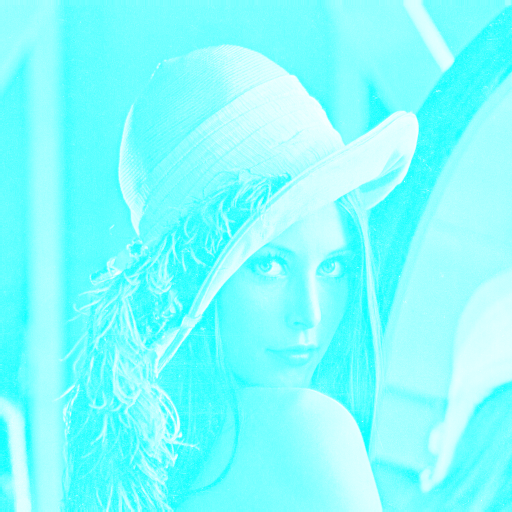
\includegraphics[width=\linewidth]{img/06/lena-CMJN-cyan}\\
      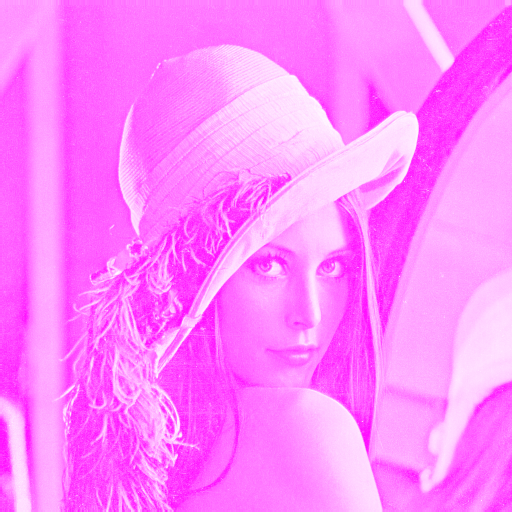
\includegraphics[width=\linewidth]{img/06/lena-CMJN-magenta}\\
      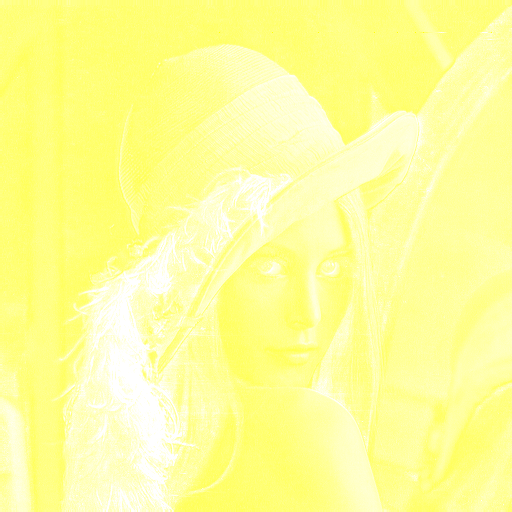
\includegraphics[width=\linewidth]{img/06/lena-CMJN-jaune}\\
      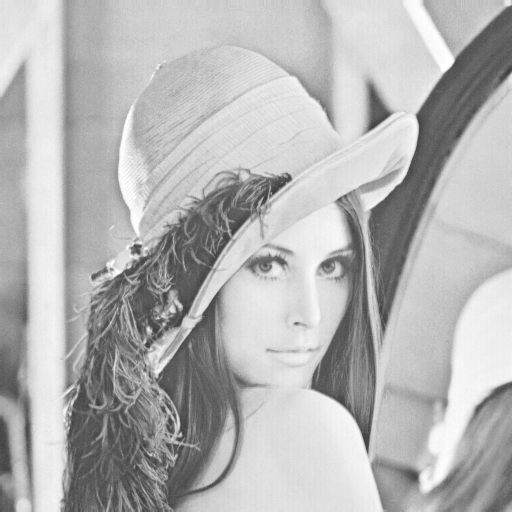
\includegraphics[width=\linewidth]{img/06/lena-CMJN-noir}\\
    \end{column}
  \end{columns}
\end{frame}
\begin{exercice}
  \begin{exercicelet}{Conversion HTML-CMJ}
    La trichromie consiste à n'utiliser que trois couleurs et faire le noire
    par mélange des autres couleurs. Dans ce cas, la formule est simple: la
    proportion d'une encre est 100\% - la proportion de la couleur
    complémentaire.

    Convertissez la couleur suivante en CM: \#FA0140. Quel genre de teinte
    est-ce ?  Est-elle très saturée ?
    \begin{xcorrection}
      FFFFFF-FA0140=05FEBF en CMJ. Elle est assez saturée (beaucoup d'encre
      magenta et pas mal de jaune). C'est quelque chose assez rouge (un peu
      violacé).
    \end{xcorrection}
  \end{exercicelet}
  \begin{exercicelet}{Vitesse d'impression}
    Une imprimante en quadrichromie est capable d'imprimer 6 pages par
    minutes, en 1200 points par pouce en mode RVB 8 bits par composante. Pour
    simplifier, on considérera qu'il y a une surface de 10 pouces × 6 pouces
    imprimable. Quelle est la quantité d'information qu'on doit fournier à
    l'imprimante pour une page ? Pour une minute d'impression ?
    \begin{xcorrection}
      Même chose que précédemment, mais seulement 8 bits, donc chaque page
      représente : 259 200 000 octets, soit environ 1,5 Go par minute.
    \end{xcorrection}
  \end{exercicelet}
\end{exercice}
\subsection{Les sons}
\begin{frame}{Qu'est-ce qu'un son?}
  Un son est une vibration de l'air transportant un signal. C'est aussi le
  signal véhiculé par vibration.

  Le son est donc numérisé comme vu au chapitre 1. Il est caractérisé par son
  spectre de fréquence instantané (les sons purs et périodiques qui le
  constituent à un moment donné). Un son est venu, à un instant donné, comme
  la somme de plusieurs sons «~purs~».
  
  La reproduction du son se fait en reproduisant une vibration qui a les mêmes
  caractéristiques fréquentielles. Les données audio sont donc des variations
  de pression (ou plutôt d'intensité électrique dans les capteurs et
  émetteurs).
\end{frame}
\begin{frame}{Les formats}
  \begin{itemize}
  \item Il faut distinguer les formats de fichiers des codecs (méthode de
    compression et filtrage des données).
  \item On distingue trois types de formats:
    \begin{enumerate}
    \item Des formats non compressés qui rajoutent quelques méta-données (ou
      pas) à des données brutes (WAV, PCM, AIFF)
    \item Des formats compressés qui utilisent un algorithme (le \emph{codec})
      pour compresser et éventuellement réduire la quantité d'information avec
      une perte acceptable de qualité (FLAC, MP3, AAC, OGG)
    \item Des formats synthétiques qui contiennent des données d'instruments
      pour reproduire de la musique à base d'une partition (MIDI, SID)
    \end{enumerate}
  \item[\ddialogwarning] Dans le domaine de la musique, le codec sert rarement
    à plusieurs formats (aucun obstacle théorique) à part PCM (pas de
    compression)
  \end{itemize}
  \begin{block}{Caractéristiques}
    Le débit d'information va dépendre:
    \begin{itemize}
    \item Du nombre de voies (émetteurs indépendants pour reconstituer
      l'aspect spatial)
    \item Des fréquences reproduites (théorème d'échantillonage)
    \item De la quantification désirée (en nombre de bits)
    \end{itemize}
  \end{block}
\end{frame}
\begin{exercice}
  \begin{exercicelet}{Compression audio MP3}
    Le codec MP3 permet de compresser le signal sonore dans une grande variété
    de débits finaux (après compression), le plus commun étant 128 kb/s. La
    fréquence d'échantillonage est quasi-toujours 44,1
    kHz. \textbf{Calculatrice autorisée}.
    \begin{questions}
    \item Quel est le débit non compressé pour de l'audio stéréo 16 bits ?
      \begin{correction}
        16 bit/sample × 44100 samples/second × 2 channels / 1000
        bits/kilobit=1411,2 kb/s.
      \end{correction}
    \item Quel est le taux de compression du format MP3 le plus classique
      (débit final 128 kb/s) ?
      \begin{correction}
        1411,2/128=11,02 (et des poussières)
      \end{correction}
    \item Et avec le format plus généreux à 320 kb/s au final?
      \begin{correction}
        1411,2/320=4,41
      \end{correction}
    \end{questions}
  \end{exercicelet}
\end{exercice}
\subsection{Les films}
\begin{frame}{Qu'est-ce qu'un film?}
  \begin{itemize}
  \item Un film est toute sorte d'image animée synchronisée ou non avec du son
    ou du texte.
  \item[\dialogwarning] Ils représentent plus de la moitié du trafic
    nord-américain sur internet.
  \item Les images successives s'appellent des trames (anglais \emph{frames}).
  \item La synchronisation avec le son doit être précise et résistante aux
    erreurs.
  \end{itemize}
\end{frame}
\begin{frame}{Les containers et les codecs}
  \begin{itemize}
  \item Comme pour l'audio, on distingue les formats (AVI, MP4, MPEG, MOV,
    MKS) des codecs (DIVX, x264, Theora, FFMPEG, Sorenson)
  \item Un certain nombre de formats n'acceptent qu'un nombre restreint de
    codecs vidéos ou audios (MP4 par exemple).
  \item Le processus administratif de normalisation pèse très lourd, car les
    fabriquants doivent faire du matériel conforme
  \item Les DRM sont des protections rajoutées qui empêchent dans certaines
    (nombreuses) circonstances d'accéder aux données. Elles sont dépendantes
    d'une inviolabilité du matériel et du logiciel.
  \item Citons aussi les GIF animés (et APNG) qui sont des formats d'images
    permettant une animation simple
  \item Ces formats peuvent contenir des méta-données plus ou moins riches
    (titre, auteurs, DRM,\dots).
  \end{itemize}
\end{frame}
\begin{frame}{L'encodage}
  \begin{itemize}
  \item La phase d'encodage d'une vidéo ou d'un fichier audio consiste à
    repérer les similarités entre plusieurs trames successives.
  \item On peut par exemple décider s'il vaut mieux décrire les différences ou
    envoyer une nouvelle image.
  \item Deux images très similaires peuvent être compressées par exemple en
    faisant un XOR binaire entre les deux et en compression RLE après.
  \item Les codecs font aussi du filtrage perceptuel pour réduire la quantité
    de données. La compression peut-être plus agressive lorsque l'autre
    méthode donne de mauvais résultats.
  \item Il est important de garder des trames complètes périodiquement pour
    gérer les erreurs.
  \item Encodage souvent en deux passes (estimation des débits binaires
    voulus, puis calcul définitif)
  \item Actuellement, l'une des opérations les plus coûteuses en temps de
    calcul.
  \item Certains formats spéciaux multi-débits permettent de s'adapter à la
    vitesse de communication de deux ordinateurs pour proposer la meilleure
    qualité \emph{(streaming)}.
  \end{itemize}
\end{frame}

% Local Variables:
% TeX-master: "archi06"
% TeX-PDF-mode: t
% fill-column: 78
% coding: utf-8-unix
% mode-require-final-newline: t
% mode: latex
% mode: flyspell
% ispell-local-dictionary: "francais"
% End:
